\subsection*{Đề thi thử THPTQG Trường An Phước, Khánh HOà, Lần 1}
\caulc
\Opensolutionfile{ans}[ans/ans-71-26-2-KhanhHoa-AnPhuoc-L1]
\begin{ex}%[1D5H2-2]
	Khảo sát thời gian đọc sách trong tuần (đơn vị: giờ) của $40$ học sinh, ta thu được bảng mẫu số liệu ghép nhóm sau:
	\begin{center}
		\begin{tabular}{|c|c|c|c|c|c|}
			\hline
			Thời gian (giờ) & $[0;2)$ & $[2;4)$ & $[4;6)$ & $[6;8)$ & $[8;10)$ \\ \hline
			Số học sinh & $5$ & $9$ & $12$ & $10$ & $4$ \\ \hline
		\end{tabular}
	\end{center}
	Trung vị của mẫu số liệu ghép nhóm trên bằng
	\choice
	{\True $5{,}0$}
	{$4{,}5$}
	{$5{,}5$}
	{$4{,}0$}
	\loigiai{
		Cỡ mẫu là $n = 40$. Vị trí của trung vị là $\dfrac{n}{2} = 20$.\\
		Tần số tích lũy của các nhóm lần lượt là: $cf_1 = 5, cf_2 = 14, cf_3 = 26, cf_4 = 36, cf_5 = 40$.\\
		Vì $14 < 20 \le 26$ nên nhóm chứa trung vị là nhóm thứ ba: $[4;6)$.\\
		Áp dụng công thức tính trung vị: $M_e = a + \dfrac{\dfrac{n}{2} - cf_{k-1}}{m_k} \cdot h$, ta có:
		\[M_e = 4 + \dfrac{20 - 14}{12} \cdot 2 = 4 + \dfrac{6}{12} \cdot 2=4 + 1=5.\]
		Vậy trung vị của mẫu số liệu là $5{,}0$.\\
	}
\end{ex}

\begin{ex}%[2H5H3-3]
	Trong không gian $Oxyz$, cho hai điểm $A(2;1;-1)$ và $B(0;3;1)$. Phương trình mặt cầu đường kính $AB$ là
	\choice
	{$(x + 1)^2 + (y + 2)^2 + z^2 = 12$}
	{$(x - 1)^2 + (y - 2)^2 + z^2 = 12$}
	{\True $(x - 1)^2 + (y - 2)^2 + z^2 = 3$}
	{$(x + 1)^2 + (y + 2)^2 + z^2 = 3$}
	\loigiai{
		Tâm $I$ của mặt cầu là trung điểm của đoạn thẳng $AB$, suy ra $I(1;2;0)$.\\
		Ta có véc-tơ $\vec{AB} = (-2;2;2)$, suy ra đường kính $AB = \sqrt{(-2)^2 + 2^2 + 2^2} = \sqrt{12} = 2\sqrt{3}$.\\
		Bán kính mặt cầu là $R = \dfrac{AB}{2} = \sqrt{3} \Rightarrow R^2 = 3$.\\
		Vậy phương trình mặt cầu là: $(x - 1)^2 + (y - 2)^2 + z^2 = 3$.
	}
\end{ex}

\begin{ex}%[2H5H2-3]
	Trong không gian $Oxyz$, phương trình chính tắc của đường thẳng đi qua hai điểm $M(1;-2;3)$ và $N(2;0;1)$ là
	\choice
	{$\dfrac{x - 2}{1} = \dfrac{y}{-2} = \dfrac{z - 1}{3}$}
	{$\dfrac{x - 1}{1} = \dfrac{y + 2}{-2} = \dfrac{z - 3}{2}$}
	{$\dfrac{x - 1}{3} = \dfrac{y + 2}{-2} = \dfrac{z - 3}{4}$}
	{\True $\dfrac{x - 1}{1} = \dfrac{y + 2}{2} = \dfrac{z - 3}{-2}$}
	\loigiai{
		Đường thẳng $MN$ nhận véc-tơ $\vec{MN} = (1;2;-2)$ làm một véc-tơ chỉ phương.\\
		Kết hợp với việc đi qua điểm $M(1;-2;3)$, ta có phương trình chính tắc: $\dfrac{x - 1}{1} = \dfrac{y + 2}{2} = \dfrac{z - 3}{-2}$.
	}
\end{ex}

\begin{ex}%[1H8H6-2]
	\immini{
	Cho hình chóp $S.ABC$ có đáy $ABC$ là tam giác vuông tại $B$, cạnh bên $SA$ vuông góc với mặt phẳng đáy. Biết $SA = a$ và $AB = a\sqrt{3}$ (tham khảo hình vẽ). Số đo góc phẳng nhị diện $[S,BC,A]$ bằng
	\choice
	{$90^\circ$}
	{$60^\circ$}
	{$45^\circ$}
	{\True $30^\circ$}}
	{
	\begin{tikzpicture}[scale=.5,>=stealth, font=\footnotesize, line join=round, line cap=round]
	\foreach \x/\y/\p in {0/0/A,1.2/-1.5/B,4/0/C}{\path (\x,\y) coordinate (\p);}
	\path ($(A)+(0,3)$) coordinate (S);
	\draw (S)--(A)--(B)--(C)--(S)--(B);
	\draw[dashed](A)--(C);
	\draw pic[draw,angle radius=2.7mm] {right angle = S--A--B};
	\draw pic[draw,angle radius=2.7mm] {right angle = S--A--C};
	\draw pic[draw,angle radius=2.7mm] {right angle = C--B--A};
	\foreach \x/\g in {A/-170,B/-110,C/-10,S/90}\fill (\x) circle (.035)+(\g:.3) node{$\x$};
\end{tikzpicture}
	}
	\loigiai{
			Góc nhị diện $[S,BC,A]$ có cạnh là đường thẳng $BC$.\\
			Ta có $BC \perp AB$ (do $\triangle ABC$ vuông tại $B$) và $BC \perp SA$ (do $SA \perp (ABC)$).\\
			Suy ra $BC \perp (SAB) \Rightarrow BC \perp SB$.\\
			Vì $AB \perp BC$ và $SB \perp BC$ nên $\widehat{SBA}$ chính là góc phẳng nhị diện của góc nhị diện $[S,BC,A]$.\\
			Xét tam giác vuông $SAB$ vuông tại $A$, ta có:
			\allowdisplaybreaks
			\begin{eqnarray*}
				\tan\widehat{SBA} = \dfrac{SA}{AB} = \dfrac{a}{a\sqrt{3}} = \dfrac{1}{\sqrt{3}} \Rightarrow \widehat{SBA} = 30^\circ.
			\end{eqnarray*}
	}
\end{ex}

\begin{ex}%[2H2H1-2]
	\immini{
	Cho hình hộp $ABCD.A'B'C'D'$ (tham khảo hình vẽ). Véc-tơ tổng $\vec{AB} + \vec{AD} + \vec{AA'}$ bằng véc-tơ nào dưới đây?
	\choice
	{$\vec{A'C}$}
	{\True $\vec{AC'}$}
	{$\vec{BD'}$}
	{$\vec{AC}$}}
	{\begin{tikzpicture}[scale=0.5,>=stealth, font=\footnotesize, line join=round, line cap=round]
	\foreach \x/\y/\p in {0/0/A,-1.1/-1.3/B,2/-1.3/C}{\path (\x,\y) coordinate (\p);}
	\path ($(A)+(C)-(B)$) coordinate (D)
	($(A)+(0.7,2.5)$)coordinate (A');
	\foreach \x/\y in {B/B',C/C',D/D'}{\path ($(A')+(\x)-(A)$) coordinate (\y);}
	\draw (C)--(C')(B')--(A')--(D')--(C')--(B')--(B)--(C)--(D)--(D');
	\draw[dashed] (A')--(A)--(D)(A)--(B);
	\foreach \x/\g in {A/-170,B/-120,C/-50,D/-10,A'/170,B'/-145,C'/-30,D'/10}\fill (\x) circle (.035)+(\g:.3) node{$\x$};
\end{tikzpicture}}
	\loigiai{
			Theo quy tắc hình hộp, ta có tổng ba véc-tơ xuất phát từ cùng một đỉnh bằng véc-tơ đường chéo không gian xuất phát từ đỉnh đó.\\
			Do vậy: $\vec{AB} + \vec{AD} + \vec{AA'} = \vec{AC'}$.
	}
\end{ex}

\begin{ex}%[2D1H4-1]
	Đường tiệm cận xiên của đồ thị hàm số $y = \dfrac{2x^2 - x + 2}{x + 1}$ là đường thẳng có phương trình
	\choice
	{\True $y = 2x - 3$}
	{$y = x - 1$}
	{$y = 2x$}
	{$y = 2x + 1$}
	\loigiai{
		Thực hiện phép chia đa thức, ta có: $y = \dfrac{2x^2 - x + 2}{x + 1} = 2x - 3 + \dfrac{5}{x + 1}$.\\
		Vì $\lim\limits_{x \to \pm\infty} [y - (2x - 3)] = \lim\limits_{x \to \pm\infty} \dfrac{5}{x + 1} = 0$ nên đường thẳng $y = 2x - 3$ là tiệm cận xiên của đồ thị hàm số.
	}
\end{ex}

\begin{ex}%[1D6H4-3]
	Tập nghiệm của bất phương trình $\log_3(x - 2) \le 2$ là
	\choice
	{$(-\infty;11]$}
	{$(2;8]$}
	{\True $(2;11]$}
	{$[2;11]$}
	\loigiai{
		Điều kiện xác định: $x - 2 > 0 \Leftrightarrow x > 2$.\\
		Bất phương trình đã cho tương đương: $x - 2 \le 3^2 \Leftrightarrow x - 2 \le 9 \Leftrightarrow x \le 11$.\\
		Kết hợp với điều kiện, ta được tập nghiệm là $S = (2;11]$.
	}
\end{ex}

\begin{ex}%[2D4H1-4]
	Họ tất cả các nguyên hình của hàm số $f(x) = 2x + \mathrm{e}^x$ là
	\choice
	{\True $x^2 + \mathrm{e}^x + C$}
	{$x^2 - \mathrm{e}^x + C$}
	{$2 + \mathrm{e}^x + C$}
	{$x^2 + \mathrm{e}^x \ln x + C$}
	\loigiai{
		Áp dụng các công thức nguyên hàm cơ bản, ta có: $\displaystyle\int (2x + \mathrm{e}^x) \mathrm{\,d}x = x^2 + \mathrm{e}^x + C$.
	}
\end{ex}

\begin{ex}%[1D2H3-6]
	Cho cấp số nhân $(u_n)$ có số hạng đầu $u_1 = 3$ và công bội $q = 2$. Tổng của $5$ số hạng đầu tiên của cấp số nhân đó bằng
	\choice
	{\True $93$}
	{$48$}
	{$45$}
	{$96$}
	\loigiai{
		Áp dụng công thức tính tổng $n$ số hạng đầu tiên của cấp số nhân: $S_n = u_1 \dfrac{1 - q^n}{1 - q}$.\\
		Ta có:
		\allowdisplaybreaks
		\begin{eqnarray*}
			S_5 = 3 \cdot \dfrac{1 - 2^5}{1 - 2} = 3 \cdot \dfrac{1 - 32}{-1} = 3 \cdot 31 =93.
		\end{eqnarray*}
	}
\end{ex}

\begin{ex}%[1H4H5-2]
	\immini{
	Cho hình lăng trụ $ABC.A'B'C'$ (tham khảo hình vẽ). Mặt phẳng $(ABC)$ song song với mặt phẳng nào dưới đây?
	\choice
	{$(ACC'A')$}
	{\True $(A'B'C')$}
	{$(ABB'A')$}
	{$(BCC'B')$}}
	{\begin{tikzpicture}[scale=0.7,>=stealth, line join=round, line cap=round, declare function={a=2.8; b=1.4; h=2.5; goc=-65; goc_xien=70;}]
			\path
			(0,0) coordinate (A)
			(goc:b) coordinate (B)
			(0:a) coordinate (C)
			(goc_xien:h) coordinate (A')
			($(A')+(B)-(A)$) coordinate (B')
			($(A')+(C)-(A)$) coordinate (C');
			\draw[dashed] (A)--(C);
			\draw (A')--(B')--(C')--cycle (B)--(C)--(C')--(B')--cycle (B)--(A)--(A');
			\foreach \x/\g in {A/-170,B/-135,C/-45,A'/90,B'/180,C'/0}
			\fill (\x) circle (.035)+(\g:.3) node{$\x$};
	\end{tikzpicture}}
	\loigiai{
			Theo tính chất cơ bản của hình lăng trụ, hai mặt đáy luôn song song với nhau.\\
			Do đó, mặt phẳng đáy $(ABC)$ song song với mặt phẳng đáy $(A'B'C')$.
	}
\end{ex}

\begin{ex}%[2D3N3-1]
	Cho hai hàm số $y = f(x)$ và $y = g(x)$ liên tục trên đoạn $[a{;}b]$. Diện tích $S$ của hình phẳng giới hạn bởi đồ thị của hai hàm số đó và hai đường thẳng $x = a, x = b$ được tính theo công thức nào dưới đây?
	\choice
	{$S = \pi \displaystyle\int\limits_a^b |f(x) - g(x)| \mathrm{\,d}x$}
	{$S = \left|\displaystyle\int\limits_a^b [f(x) - g(x)] \mathrm{\,d}x\right|$}
	{$S = \displaystyle\int\limits_a^b [f(x) - g(x)] \mathrm{\,d}x$}
	{\True $S = \displaystyle\int\limits_a^b |f(x) - g(x)| \mathrm{\,d}x$}
	\loigiai{
		Công thức tính diện tích hình phẳng giới hạn bởi hai đồ thị hàm số $y = f(x), y = g(x)$ và các đường thẳng $x = a, x = b$ là $S = \displaystyle\int\limits_a^b |f(x) - g(x)| \mathrm{\,d}x$.
	}
\end{ex}

\begin{ex}%[1D1H5-3]
	Nghiệm của phương trình $2\cos x = 1$ là
	\choice
	{\True $x = \pm\dfrac{\pi}{3} + k2\pi\ (k \in \mathbb{Z})$}
	{$x = \pm\dfrac{\pi}{3} + k\pi\ (k \in \mathbb{Z})$}
	{$x = \pm\dfrac{\pi}{6} + k\pi\ (k \in \mathbb{Z})$}
	{$x = \pm\dfrac{\pi}{6} + k2\pi\ (k \in \mathbb{Z})$}
	\loigiai{
		Ta có $\cos x = \dfrac{1}{2} \Leftrightarrow \cos x = \cos\dfrac{\pi}{3} \Leftrightarrow x = \pm\dfrac{\pi}{3} + k2\pi\ (k \in \mathbb{Z})$.
	}
\end{ex}
\Closesolutionfile{ans}

\cauds
\Opensolutionfile{ans}[ans/ans-71-26-2-KhanhHoa-AnPhuoc-L1-DS]
\begin{ex}%[2D6V2-4]
	Tại một bệnh viện, người ta áp dụng một phương pháp xét nghiệm rà soát nhanh đối với một loại Virus X. Dữ liệu thống kê y tế cho thấy tỉ lệ người dân thực sự nhiễm loại Virus này trong cộng đồng là $2\%$. Khả năng của bộ xét nghiệm như sau: Nếu một người thực sự nhiễm Virus X, xét nghiệm sẽ cho kết quả dương tính với xác suất $95\%$; nhưng nếu một người không nhiễm bệnh, xét nghiệm vẫn có thể báo dương tính (dương tính giả) với xác suất $4\%$. Chọn ngẫu nhiên một người tham gia rà soát. Gọi $A$ là biến cố "Người đó thực sự nhiễm Virus X" và $B$ là biến cố "Người đó có kết quả xét nghiệm dương tính".
	\choiceTF
	{\True Xác suất một người bất kỳ nhận kết quả dương tính là $0{,}0582$}
	{Xác suất một người nhận kết quả xét nghiệm dương tính biết rằng người đó không nhiễm bệnh là $0{,}96$}
	{\True $P(A) = 0{,}02$ và $P(B|A) = 0{,}95$}
	{Nếu một người cầm trên tay tờ kết quả dương tính, khả năng người đó thực sự mắc bệnh là rất cao (trên $50\%$), do đó bác sĩ có thể lập tức đưa người này vào phác đồ điều trị mạnh}
	\loigiai{
		\begin{itemchoice}
			\itemch \textbf{Đúng.} Ta có $P(\overline{A}) = 1 - P(A) = 1 - 0{,}02 = 0{,}98$. Sử dụng công thức xác suất toàn phần, xác suất có kết quả dương tính là:
			\allowdisplaybreaks
			\begin{eqnarray*}
				P(B) &=& P(A) \cdot P(B|A) + P(\overline{A}) \cdot P(B|\overline{A})\\
				&=& 0{,}02 \times 0{,}95 + 0{,}98 \times 0{,}04 = 0{,}0190 + 0{,}0392 = 0{,}0582.
			\end{eqnarray*}
			\itemch \textbf{Sai.} Biến cố "người đó không nhiễm bệnh" là $\overline{A}$. Việc xét nghiệm ra dương tính với người không bệnh (dương tính giả) là $4\%$. Do đó, ta có $P(B|\overline{A}) = 0{,}04$.
			\itemch \textbf{Đúng.} Theo thống kê, có $2\%$ người dân nhiễm bệnh nên $P(A) = 0{,}02$. Xác suất xét nghiệm dương tính khi người đó có bệnh là $95\%$ nên $P(B|A) = 0{,}95$.
			\itemch \textbf{Sai.} Cần tính xác suất người đó thực sự mắc bệnh khi đã có kết quả dương tính, tức là $P(A|B)$. Áp dụng công thức Bayes:
			\begin{eqnarray*}
				P(A|B) = \dfrac{P(A) \cdot P(B|A)}{P(B)} = \dfrac{0{,}0190}{0{,}0582} = \dfrac{190}{582} \approx 0{,}3265 = 32{,}65\%.
			\end{eqnarray*}
		\end{itemchoice}
	}
\end{ex}

\begin{ex}%[2D1H3-1]
	Cho hàm số $y = f(x) = \dfrac{x^2 - 3x + 3}{x - 1}$.
	\choiceTF
	{Đạo hàm của hàm số là $f'(x) = \dfrac{x^2 - 2x}{(x - 1)^2}$}
	{Hàm số đã cho nghịch biến trên khoảng $(0;2)$}
	{Điểm cực tiểu của đồ thị hàm số là $(2;1)$}
	{Giá trị lớn nhất của hàm số trên đoạn $[-2;0]$ bằng $0$}
	\loigiai{
		\begin{itemchoice}
			\itemch \textbf{Đúng.} Ta có $f'(x) = \dfrac{(2x - 3)(x - 1) - (x^2 - 3x + 3)}{(x - 1)^2} = \dfrac{x^2 - 2x}{(x - 1)^2}$.\\
			Cho $f'(x) = 0 \Leftrightarrow x^2 - 2x = 0 \Leftrightarrow x = 0$ hoặc $x = 2$. Cả hai nghiệm đều thỏa mãn điều kiện $x \ne 1$.
			\itemch \textbf{Sai.} Ta có $f'(x) < 0 \Leftrightarrow \left\{\begin{aligned} &x^2 - 2x < 0 \\ &x \ne 1 \end{aligned}\right. \Leftrightarrow \left\{\begin{aligned} &0 < x < 2 \\ &x \ne 1. \end{aligned}\right.$\\
			Hàm số nghịch biến trên các khoảng $(0;1)$ và $(1;2)$. Không thể kết luận nghịch biến trên khoảng $(0;2)$ vì hàm số gián đoạn tại $x = 1$.
			\itemch \textbf{Đúng.} Bảng xét dấu $f'(x)$ cho thấy $f'(x)$ đổi dấu từ âm sang dương khi qua $x = 2$.\\
			Do đó hàm số đạt cực tiểu tại $x = 2$. Giá trị cực tiểu $f(2) = 1$. Suy ra điểm cực tiểu của đồ thị hàm số là $(2;1)$.
			\itemch \textbf{Sai.} Xét hàm số trên đoạn $[-2;0]$. Ta thấy trên đoạn này $x \le 0 \Rightarrow x^2 - 2x \ge 0$, do đó $f'(x) \ge 0$, hàm số đồng biến.\\
			Giá trị lớn nhất trên đoạn $[-2;0]$ là $f(0) = -3$ (không phải bằng $0$).
		\end{itemchoice}
	}
\end{ex}

\begin{ex}%[2H5V4-5]
	Trong không gian với hệ trục tọa độ $Oxyz$ (đơn vị đo trên các trục là mét), một thiết bị lặn không người lái xuất phát từ điểm $A(1;1;1)$. Thiết bị lặn di chuyển theo một quỹ đạo là đường thẳng với hướng luôn được xác định bởi véc-tơ $\vec{u} = (2;2;1)$. Biết rằng tốc độ di chuyển của thiết bị tại thời điểm $t$ (giây) kể từ lúc xuất phát được mô phỏng bởi hàm số $v(t) = 2t + 2$ (m/s).
	\choiceTF
	{Mặt phẳng đi qua điểm xuất phát $A$ và vuông góc với quỹ đạo chuyển động của thiết bị lặn có phương trình tổng quát là $2x + 2y + z - 5 = 0$}
	{Quãng đường thiết bị lặn di chuyển được sau $3$ giây đầu tiên kể từ lúc xuất phát là $15$ mét}
	{Phương trình chính tắc của đường thẳng mô tả quỹ đạo chuyển động của thiết bị lặn là $\dfrac{x - 2}{1} = \dfrac{y - 2}{1} = \dfrac{z - 1}{1}$}
	{\True Giả sử vùng cảnh báo an ninh của một trạm quan sát ngầm là khối cầu $(S) \colon x^2 + y^2 + z^2 - 22x - 22y + 217 \le 0$. Tại thời điểm $t = 3$ (giây), thiết bị lặn vẫn nằm ngoài vùng cảnh báo an ninh này}
	\loigiai{
		\begin{itemchoice}
			\itemch \textbf{Đúng.} Quỹ đạo chuyển động của thiết bị lặn là đường thẳng nhận $\vec{u} = (2;2;1)$ làm véc-tơ chỉ phương. Do đó, mặt phẳng vuông góc với quỹ đạo sẽ nhận $\vec{n} = \vec{u} = (2;2;1)$ làm véc-tơ pháp tuyến.\\
			Phương trình mặt phẳng đi qua $A(1;1;1)$ có dạng:
			\[ 2(x - 1) + 2(y - 1) + 1(z - 1) = 0 \Leftrightarrow 2x + 2y + z - 5 = 0. \]
			\itemch \textbf{Đúng.} Quãng đường thiết bị lặn di chuyển được sau $3$ giây đầu tiên được tính bằng tích phân của hàm vận tốc:
			\[ S = \displaystyle\int\limits_0^3 v(t) \mathrm{\,d}t = \displaystyle\int\limits_0^3 (2t + 2) \mathrm{\,d}t = \left[t^2 + 2t\right]_0^3 = 3^2 + 2(3) = 15\text{ (mét)}. \]
			\itemch \textbf{Sai.} Đường thẳng mô tả quỹ đạo đi qua điểm $A(1;1;1)$ và có véc-tơ chỉ phương $\vec{u} = (2;2;1)$ nên phương trình chính tắc là $\dfrac{x - 1}{2} = \dfrac{y - 1}{2} = \dfrac{z - 1}{1}$.
			\itemch \textbf{Đúng.} Tại thời điểm $t = 3$, quãng đường thiết bị lặn đi được là $S = 15$ m. Gọi $M$ là vị trí của thiết bị lúc này. Vì thiết bị di chuyển thẳng từ $A$ theo hướng của véc-tơ $\vec{u}$ nên véc-tơ độ dời $\vec{AM}$ sẽ cùng hướng với $\vec{u}$.\\
			Độ dài của $\vec{u}$ là $|\vec{u}| = \sqrt{2^2 + 2^2 + 1^2} = 3$.\\
			Ta có mối liên hệ: $\vec{AM} = \dfrac{S}{|\vec{u}|} \vec{u} = \dfrac{15}{3}(2;2;1) = 5(2;2;1) = (10;10;5)$.\\
			Suy ra tọa độ điểm $M$ là: $M = A + \vec{AM} = (1 + 10; 1 + 10; 1 + 5) = (11;11;6)$.\\
			Khối cầu vùng cảnh báo có bất phương trình $x^2 + y^2 + z^2 - 22x - 22y + 217 \le 0$.\\
			Từ phương trình này, ta xác định được tâm $I\left(-\dfrac{-22}{2}; -\dfrac{-22}{2}; 0\right) = I(11;11;0)$ và bán kính $R = \sqrt{11^2 + 11^2 + 0^2 - 217} = \sqrt{242 - 217} = \sqrt{25} = 5$.\\
			Khoảng cách từ $M$ đến tâm $I$ là:
			\[ IM = \sqrt{(11 - 11)^2 + (11 - 11)^2 + (6 - 0)^2} = \sqrt{36} = 6. \]
			Vì $IM = 6 > R = 5$, nên tại thời điểm $t = 3$ (giây), thiết bị lặn vẫn chưa đi vào phần không gian bên trong của khối cầu cảnh báo (nằm ngoài).
		\end{itemchoice}
	}
\end{ex}

\begin{ex}%[1D6V3-5]
	Trong một môi trường nuôi cấy thí nghiệm, số lượng vi khuẩn $N(t)$ (con) sau thời gian $t$ (giờ) sinh sôi với tốc độ tỉ lệ thuận với số lượng vi khuẩn hiện có, tức là thỏa mãn phương trình đạo hàm $N'(t) = k \cdot N(t)$ (với $k$ là hằng số sinh trưởng). Biết rằng ban đầu ($t = 0$) có $500$ con vi khuẩn và sau $3$ giờ thì số lượng vi khuẩn tăng lên thành $4000$ con.
	\choiceTF
	{\True Hàm số có dạng $N(t) = A \cdot \mathrm{e}^{kt}$ (với $A > 0$ là hằng số)}
	{Số lượng vi khuẩn có trong môi trường nuôi cấy sau $6$ giờ là $16\,000$ con}
	{\True $A = 500$ và $k = \ln 2$}
	{\True Sau nửa ngày nuôi cấy, số lượng vi khuẩn sẽ vượt qua mốc $2$ triệu con}
	\loigiai{
		\begin{itemchoice}
			\itemch \textbf{Đúng.} Ta có $\dfrac{N'(t)}{N(t)} = k \Rightarrow \displaystyle\int \dfrac{N'(t)}{N(t)} \mathrm{\,d}t = \displaystyle\int k \mathrm{\,d}t \Rightarrow \ln|N(t)| = kt + C_1$.\\
			Vì số lượng vi khuẩn $N(t) > 0$ nên $N(t) = \mathrm{e}^{kt+C_1} = \mathrm{e}^{C_1} \cdot \mathrm{e}^{kt} = C \cdot \mathrm{e}^{kt}$ (với $C = \mathrm{e}^{C_1} > 0$).
			\itemch \textbf{Sai.} Từ kết quả tìm được ở ý c), hàm số mô hình là $N(t) = 500 \cdot \mathrm{e}^{t \ln 2} = 500 \cdot 2^t$.\\
			Sau $6$ giờ ($t = 6$), số lượng vi khuẩn là $N(6) = 500 \cdot 2^6 = 500 \cdot 64 = 32\,000$ (con) chứ không phải $16\,000$.
			\itemch \textbf{Đúng.} Thời điểm ban đầu $t = 0$, ta có $N(0) = 500 \Rightarrow C \cdot \mathrm{e}^0 = 500 \Rightarrow C = 500$.\\
			Sau $3$ giờ, $N(3) = 4000 \Rightarrow 500 \cdot \mathrm{e}^{3k} = 4000 \Rightarrow \mathrm{e}^{3k} = 8 \Rightarrow \mathrm{e}^k = 2 \Rightarrow k = \ln 2$.
			\itemch \textbf{Đúng.} Nửa ngày tương đương với $t = 12$ giờ.\\
			Số lượng vi khuẩn tại thời điểm này là $N(12) = 500 \cdot 2^{12} = 500 \cdot 4096 = 2\,048\,000$ (con).\\
			Vì $2\,048\,000 > 2\,000\,000$ nên số lượng vi khuẩn đã vượt mốc $2$ triệu con.
		\end{itemchoice}
	}
\end{ex}
\Closesolutionfile{ans}

\caukq
\Opensolutionfile{ans}[ans/ans-71-26-2-KhanhHoa-AnPhuoc-L1-KQ]
\begin{ex}%[0D8V2-5]
	Trong đợt phòng chống dịch, một bệnh viện trung ương cần phân bổ khẩn cấp $15$ thùng vật tư y tế (các thùng giống hệt nhau) cho $3$ trạm y tế cơ sở là $A$, $B$ và $C$. Theo quy định đánh giá rủi ro, trạm $A$ phải nhận được ít nhất $4$ thùng, trạm $B$ nhận ít nhất $3$ thùng và trạm $C$ nhận ít nhất $1$ thùng. Hỏi bệnh viện có tất cả bao nhiêu cách phân bổ $15$ thùng vật tư này để thỏa mãn các yêu cầu trên?
	\shortans{36}
	\loigiai{
		Gọi $x_A, x_B, x_C$ lần lượt là số thùng vật tư phân bổ cho $3$ trạm y tế. Ta có phương trình tổng số thùng: $x_A + x_B + x_C = 15$.\\
		Điều kiện ràng buộc: $x_A \ge 4, x_B \ge 3, x_C \ge 1$ (với $x_i \in \mathbb{N}$).\\
		Đặt $y_A = x_A - 4 \ge 0, y_B = x_B - 3 \ge 0, y_C = x_C - 1 \ge 0$.\\
		Thế vào phương trình ban đầu, ta được:
		\[ (y_A + 4) + (y_B + 3) + (y_C + 1) = 15 \Leftrightarrow y_A + y_B + y_C = 7. \]
		Số cách phân bổ chính là số nghiệm nguyên không âm của phương trình $y_A + y_B + y_C = 7$.\\
		Áp dụng thuật toán chia kẹo Euler (bài toán vách ngăn) chia $n = 7$ phần tử cho $k = 3$ nhóm, số cách chia là:
		\[\mathrm{C}_{n+k-1}^{k-1} = \mathrm{C}_{7+3-1}^{3-1} = \mathrm{C}_9^2 = \dfrac{9 \times 8}{2} = 36\text{ (cách)}.\]
	}
\end{ex}

\begin{ex}%[0D8V2-5]
	Một hệ thống phân tải mạng tự động phân phối ngẫu nhiên $7$ gói dữ liệu (giống hệt nhau) cho $4$ máy chủ xử lý (được đánh số $1, 2, 3, 4$). Hệ thống được lập trình để đảm bảo mỗi máy chủ đều nhận được ít nhất $1$ gói dữ liệu nhằm duy trì hoạt động liên tục. Tính xác suất để máy chủ số $1$ nhận được đúng $2$ gói dữ liệu (viết kết quả dưới dạng số thập phân).
	\shortans{0,3}
	\loigiai{
		Gọi $x_1, x_2, x_3, x_4$ lần lượt là số gói dữ liệu mà $4$ máy chủ nhận được. Ta có phương trình: $x_1 + x_2 + x_3 + x_4 = 7$ với điều kiện $x_i \ge 1\ (\forall i = 1, 2, 3, 4)$.\\
		Số phần tử của không gian mẫu chính là số nghiệm nguyên dương của phương trình trên. Áp dụng bài toán chia kẹo Euler, số cách phân phối là:
		\[ n(\Omega) = \mathrm{C}_{7-1}^{4-1} = \mathrm{C}_6^3 = \dfrac{6!}{3!3!} = 20\text{ (cách)}. \]
		Gọi biến cố $A$: "Máy chủ số $1$ nhận được đúng $2$ gói dữ liệu". Khi đó $x_1 = 2$.\\
		Suy ra $x_2 + x_3 + x_4 = 7 - 2 = 5$ với $x_2, x_3, x_4 \ge 1$.\\
		Số cách phân phối cho $3$ máy chủ còn lại là số nghiệm nguyên dương của phương trình $x_2 + x_3 + x_4 = 5$, tương ứng với:
		\[ n(A) = \mathrm{C}_{5-1}^{3-1} = \mathrm{C}_4^2 = 6\text{ (cách)}. \]
		Xác suất của biến cố $A$ là:
		\[P(A) = \dfrac{n(A)}{n(\Omega)} = \dfrac{6}{20} = 0{,}3.\]
	}
\end{ex}

\begin{ex}%[2D3V3-5]
	\immini{
	Một thùng ủ rượu vang bằng gỗ sồi có dạng là một khối tròn xoay. Nếu cắt thùng bởi một mặt phẳng chứa trục đối xứng của thùng thì đường viền ngoài của thiết diện là một phần của đường parabol. Biết thùng có chiều dài $10$ dm, đường kính hai mặt đáy bằng nhau và bằng $6$ dm, phần phình to nhất ở giữa thùng có đường kính bằng $8$ dm. Hãy tính dung tích của thùng ủ rượu này (đơn vị: lít, làm tròn kết quả đến hàng đơn vị). (Biết $1\text{ lít} = 1\text{ dm}^3$ và giả sử bỏ qua độ dày của vỏ gỗ).
	\shortans{425}}
	{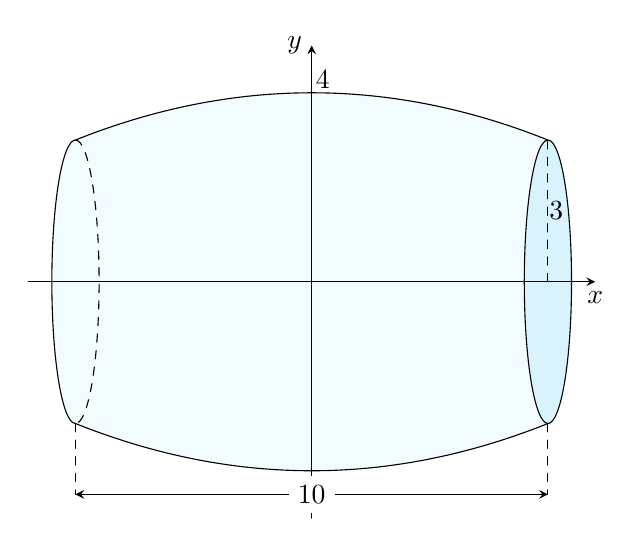
\begin{tikzpicture}[scale=0.6,>=stealth, line join=round, line cap=round, smooth, samples=450, declare function={xmin=-6; xmax=6; ymin=-5; ymax=5; a=-1/25; b=4;}]
			\path (0,0) node[below left]{$O$};
			\fill[cyan!5] plot[domain=-5:5] (\x, {a*(\x)^2+b}) -- (5,0) -- plot[domain=5:-5] (\x, {-a*(\x)^2-b}) -- (-5,-3) arc (-90:-270:0.5 and 3)--cycle;
			\draw[fill=cyan!15] (5,0) ellipse (0.5 and 3);
			\draw[dashed] (-5,3) arc (90:-90:0.5 and 3) ;
			\draw plot[domain=-5:5] (\x, {a*(\x)^2+b}) plot[domain=-5:5] (\x, {-a*(\x)^2-b})
			(-5,3) arc (90:270:0.5 and 3)
			;
			\draw[->] (xmin,0)--(xmax,0) node[below]{$x$};
			\draw[->] (0,ymin)--(0,ymax) node[left]{$y$};
			\draw[dashed] (0,0)--(0,4) node[above right=-2pt]{$4$};
			\draw[dashed] (5,0)--(5,3) node[midway,right=-3pt]{$3$};
			\draw[<->] (-5,-4.5)--(5,-4.5) node[midway,fill=white]{$10$};
			\draw[dashed] (-5,-3)--(-5,-4.5) (5,-3)--(5,-4.5);
	\end{tikzpicture}}
	\loigiai{
		\textbf{Bước 1 (Mô hình hóa):} Gắn hệ trục tọa độ $Oxy$ sao cho trục $Ox$ trùng với trục đối xứng của thùng, gốc tọa độ $O$ nằm tại vị trí chính giữa của thùng. Vì thùng dài $10$ dm nên thân thùng trải dài từ hoành độ $x = -5$ đến $x = 5$.\\
		Bán kính phần phình to nhất tại $x = 0$ là $r_{\max} = \dfrac{8}{2} = 4$ dm. Do đó, đỉnh của parabol là $(0;4)$. Phương trình parabol có dạng $y = ax^2 + 4$.\\
		Bán kính tại đáy $x = 5$ là $r = \dfrac{6}{2} = 3$ dm. Parabol đi qua điểm $(5;3)$. Thay vào phương trình:\\
		$3 = a(5)^2 + 4 \Leftrightarrow 25a = -1 \Rightarrow a = -0{,}04$.\\
		Vậy phương trình đường biên là $y = -0{,}04x^2 + 4$.\\
		\noindent\textbf{Bước 2 (Tính thể tích):} Dung tích thùng rượu là thể tích khối tròn xoay sinh ra khi quay phần hình phẳng giới hạn bởi $y = -0{,}04x^2 + 4, y = 0, x = -5, x = 5$ quanh trục $Ox$.
		\[ V = \pi \displaystyle\int\limits_{-5}^{5} (-0{,}04x^2 + 4)^2 \mathrm{\,d}x = 2\pi \displaystyle\int\limits_{0}^{5} (0{,}0016x^4 - 0{,}32x^2 + 16) \mathrm{\,d}x \]
		Tính nguyên hàm: $F(x) = 0{,}0016\dfrac{x^5}{5} - 0{,}32\dfrac{x^3}{3} + 16x$. Thay cận $x = 5$:
		\[ F(5) = 0{,}0016\left(\dfrac{3125}{5}\right) - 0{,}32\left(\dfrac{125}{3}\right) + 16(5) = 1 - \dfrac{40}{3} + 80 = 81 - \dfrac{40}{3} = \dfrac{203}{3}. \]
		Vậy $V = 2\pi \left(\dfrac{203}{3}\right) = \dfrac{406\pi}{3} \approx 425{,}16\text{ (dm}^3\text{)}$. Làm tròn đến hàng đơn vị, dung tích của thùng là $425$ lít.\\
	}
\end{ex}

\begin{ex}%[2D1V3-6]
	Một hộ làm nghề dệt vải thổ cẩm ở làng Mỹ Nghiệp thuộc xã Ninh Phước tỉnh Khánh Hòa sản xuất mỗi ngày được $x$ mét vải thổ cẩm ($1 \le x \le 18$). Tổng chi phí sản xuất $x$ mét vải thổ cẩm (tính bằng nghìn đồng) cho bởi hàm số $C(x) = x^3 - 3x^2 - 20x + 500$. Giả sử hộ làm nghề dệt thổ cẩm này bán hết sản phẩm mỗi ngày với giá $220$ nghìn đồng/mét. Hỏi hộ làm nghề dệt thổ cẩm cần sản xuất và bán ra mỗi ngày bao nhiêu mét vải thổ cẩm để thu được lợi nhuận tối đa?
	\shortans{10}
	\loigiai{
		Tổng doanh thu mỗi ngày khi bán $x$ mét thổ cẩm là:
		\[ R(x) = 220x\text{ (nghìn đồng)}. \]
		Hàm lợi nhuận mỗi ngày thu được là:
		\[ P(x) = R(x) - C(x) = 220x - (x^3 - 3x^2 - 20x + 500) = -x^3 + 3x^2 + 240x - 500. \]
		Ta cần tìm giá trị lớn nhất của hàm số $P(x)$ trên đoạn $[1{;}18]$. Đạo hàm: $P'(x) = -3x^2 + 6x + 240$.\\
		Cho $P'(x) = 0 \Leftrightarrow -3x^2 + 6x + 240 = 0 \Leftrightarrow \left[\begin{aligned} &x = 10\text{ (thỏa mãn)} \\ &x = -8\text{ (loại).} \end{aligned}\right.$\\
		Ta tính các giá trị của hàm số tại hai đầu mút và tại điểm tới hạn:
		\allowdisplaybreaks
		\begin{eqnarray*}
			P(1) &=& -(1)^3 + 3(1)^2 + 240(1) - 500 = -258.\\
			P(10) &=& -(10)^3 + 3(10)^2 + 240(10) - 500 = -1000 + 300 + 2400 - 500 = 1200.\\
			P(18) &=& -(18)^3 + 3(18)^2 + 240(18) - 500 = -5832 + 972 + 4320 - 500 = -1040.
		\end{eqnarray*}
		So sánh các giá trị, ta thấy $\max\limits_{x \in [1{;}18]} P(x) = P(10) = 1200$.\\
		Vậy hộ làm nghề dệt thổ cẩm cần sản xuất và bán ra $10$ mét vải thổ cẩm mỗi ngày để đạt lợi nhuận tối đa.
	}
\end{ex}

\begin{ex}%[1H8H5-4]
	\immini{
	Tại một khu du lịch sinh thái, người ta thiết kế một mái vòm kính có dạng hình chóp tứ giác đều $S.ABCD$. Đáy $ABCD$ là hình vuông tâm $O$ có độ dài cạnh bằng $6$ m. Cột trụ $SO$ đỡ mái vòm vuông góc với mặt sàn $(ABCD)$ và có chiều cao $4$ m. Để giăng một dải đèn LED trang trí từ cạnh đáy $AB$ sang cạnh bên $SC$, các kĩ sư cần tính toán khoảng cách ngắn nhất giữa hai thanh thép thẳng đặt dọc theo hai đường thẳng $AB$ và $SC$. Tính khoảng cách này (đơn vị: mét, viết kết quả dưới dạng số thập phân).
	\shortans{4,8}}
	{\begin{tikzpicture}[scale=1,>=stealth, line join=round, line cap=round, declare function={a=3.2; b=1.5; h=3.3; goc=-140;}]
			\path
			(0,0) coordinate (A)
			(goc:b) coordinate (B)
			(0:a) coordinate (D)
			($(B)+(D)$) coordinate (C)
			(intersection of A--C and B--D) coordinate (O)
			(O)+(0,h) coordinate (S)
			($(C)!0.5!(D)$) coordinate (H)
			(intersection of S--H and O--H) coordinate (H);
			\path ($(S)!0.62!(H)$) coordinate (K);
			\draw[dashed] (A)--(D) (A)--(C) (B)--(D) (S)--(O) (S)--(A);
			\draw[dashed, red] (A)--(B);
			\draw (S)--(B)--(C)--(D)--(S)--(C);
			\draw[blue] (S)--(C);
			\foreach \x/\g in {A/145,B/-140,C/-40,D/40,O/-90,S/90}
			\path[fill=white, draw] (\x) circle (.035)+(\g:.3) node{$\x$};
	\end{tikzpicture}}
	\loigiai{
		\immini{
			Do $AB \parallel CD \subset (SCD)$ nên $AB \parallel (SCD)$.\\
			Suy ra $\mathrm{d}(AB, SC) = \mathrm{d}(AB, (SCD)) = \mathrm{d}(A, (SCD))$.\\
			Mà $AC \cap (SCD) = C$ và $AC = 2OC$ nên:
			\[ \mathrm{d}(A, (SCD)) = 2\mathrm{d}(O, (SCD)). \]
			Gọi $H$ là trung điểm của $CD$, kẻ $OK \perp SH$ tại $K$.\\
			Vì $CD \perp OH$ và $CD \perp SO \Rightarrow CD \perp (SOH) \Rightarrow CD \perp OK$.\\
			Do đó $OK \perp (SCD) \Rightarrow \mathrm{d}(O, (SCD)) = OK$.\\
			Xét $\triangle SOH$ vuông tại $O$, đường cao $OK$:
			\[ \dfrac{1}{OK^2} = \dfrac{1}{SO^2} + \dfrac{1}{OH^2} = \dfrac{1}{4^2} + \dfrac{1}{3^2} = \dfrac{25}{144} \Rightarrow OK = 2{,}4\text{ m}. \]
			Vậy $\mathrm{d}(AB, SC) = 2 \times 2{,}4 = 4{,}8$ m.
		}{
			\begin{tikzpicture}[scale=1,>=stealth, line join=round, line cap=round, declare function={a=3.2; b=1.5; h=3.8; goc=-140;}]
				\path
				(0,0) coordinate (A)
				(goc:b) coordinate (B)
				(0:a) coordinate (D)
				($(B)+(D)$) coordinate (C)
				(intersection of A--C and B--D) coordinate (O)
				(O)+(0,h) coordinate (S)
				($(C)!0.5!(D)$) coordinate (H)
				(intersection of S--H and O--H) coordinate (H);
				\path ($(S)!0.62!(H)$) coordinate (K);
				\draw[dashed] (A)--(D) (A)--(C) (B)--(D) (S)--(O)--(H) (O)--(K) (S)--(A);
				\draw[dashed, red] (A)--(B);
				\draw (H)--(S)--(B)--(C)--(D)--(S)--(C);
				\draw[blue] (S)--(C);
				\foreach \x/\g in {A/145,B/-140,C/-40,D/40,O/-90,S/90,H/-30,K/35}
				\path[fill=white, draw] (\x) circle (.035)+(\g:.3) node{$\x$};
			\end{tikzpicture}
		}
	}
\end{ex}

\begin{ex}%[0D7V2-7]
	Một khách sạn công nghệ cao có $50$ phòng cho thuê. Nếu khách sạn đặt giá thuê mỗi phòng là $2$ triệu đồng/ngày thì toàn bộ các phòng đều được thuê hết. Nghiên cứu thị trường cho thấy, cứ mỗi lần tăng giá thuê thêm $100$ nghìn đồng/ngày thì sẽ có thêm $1$ phòng bị bỏ trống. Biết chi phí vận hành, dọn dẹp cho mỗi phòng được thuê là $200$ nghìn đồng/ngày (phòng trống không mất chi phí này). Để lợi nhuận thu được trong ngày từ việc cho thuê phòng đạt từ $115$ triệu đồng trở lên, khách sạn có thể thiết lập mức giá cho thuê cao nhất là bao nhiêu triệu đồng/ngày?
	\shortans{3,8}
	\loigiai{
		Gọi $x$ là số lần tăng giá thêm $100$ nghìn đồng ($x \in \mathbb{N}, 0 \le x \le 50$).\\
		Giá thuê mỗi phòng lúc này là: $2000 + 100x$ (nghìn đồng).\\
		Số phòng được thuê là: $50 - x$ (phòng).\\
		Hàm doanh thu: $R(x) = (2000 + 100x)(50 - x)$.\\
		Hàm chi phí: $C(x) = 200(50 - x)$.\\
		Hàm lợi nhuận:
		\[ P(x) = R(x) - C(x) = (1800 + 100x)(50 - x) = 100(18 + x)(50 - x) = 100(-x^2 + 32x + 900). \]
		Để lợi nhuận đạt từ $115$ triệu đồng ($115\,000$ nghìn đồng) trở lên:
		\[ 100(-x^2 + 32x + 900) \ge 115\,000 \Leftrightarrow -x^2 + 32x + 900 \ge 1150 \Leftrightarrow -x^2 + 32x - 250 \ge 0 \Leftrightarrow x^2 - 32x + 250 \le 0. \]
		Giải bất phương trình ta được: $16 - \sqrt{6} \le x \le 16 + \sqrt{6} \Leftrightarrow 13{,}55 \le x \le 18{,}45$.\\
		Vì khách sạn muốn đặt mức giá thuê cao nhất nên ta cần chọn $x$ lớn nhất. Với $x \in \mathbb{N}$, giá trị lớn nhất thỏa mãn là $x = 18$.\\
		Mức giá cho thuê tương ứng là: $2000 + 100(18) = 3800$ nghìn đồng $= 3{,}8$ triệu đồng/ngày.
	}
\end{ex}
\Closesolutionfile{ans}